\chapter{Propuesta}\label{chapter:proposal}

El modelo propuesto se divide en dos secciones. En la primera sección se realiza la segmentación y clasificación de 
las UDAs como tareas conjuntas. En la segunda sección se predicen los enlaces y sus clasificaciones, tomando
como tareas auxiliares la clasificación de las UDAs. Dada la heterogeniedad de las conjuntos de datos disponibles 
en EA los modelos poseen un mínimo de atributos hechos a mano, esto permite que el modelo por sí solo aprenda 
la mejor representación para el esquema de anotación con que se entrene.

\section{Segmentación y clasificacón de UDAs}

Esta primera parte se modeló como un problema secuencia a secuencia cuyo objetivo es asignar a los tokens 
extraídos del documento entrada una etiqueta BIOES para segmentar las UDAs. Para la clasificación del tipo 
de UDA al conjunto de etiquetas BIES se le añadieron las clasificaciones que presentan el corpus entrenante.

\begin{center}
    En$_O$ primer$_O$ lugar$_O$,$_O$ \emph{el$_{B-A}$ correo$_{I-A}$ electronico$_{I-A}$ puede$_{I-A}$ 
    contar$_{I-A}$ como$_{I-A}$ uno$_{I-A}$ de$_{I-A}$ los$_{I-A}$ resultados$_{I-A}$
    más$_{I-A}$ beneficiosos$_{I-A}$ de$_{I-A}$ la$_{I-A}$ tecnología$_{I-A}$ moderna$_{E-A}$}.$_{O}$ 
    \emph{Años$_{B-P}$ atrás$_{I-P}$, las$_{I-P}$ personas$_{I-P}$ pagaban$_{I-P}$ gran$_{I-P}$ cantidad$_{I-P}$ 
    de$_{I-P}$ dinero$_{I-P}$ para$_{I-P}$ enviar$_{I-P}$ sus$_{I-P}$ cartas$_{I-P}$ y$_{I-P}$ sus$_{I-P}$ 
    pagos$_{I-P}$ estaban$_{I-P}$ sujetos$_{I-P}$ al$_{I-P}$ peso$_{I-P}$ de$_{I-P}$ sus$_{I-P}$ 
    cartas$_{I-P}$ o$_{I-P}$ paquetes$_{I-P}$ y$_{I-P}$ muchos$_{I-P}$ accidentes$_{I-P}$ podrían$_{I-P}$
    causar$_{I-P}$ problemas$_{I-P}$ que$_{I-P}$ causarían$_{I-P}$ que$_{I-P}$ el$_{I-P}$ correo$_{I-P}$ 
    no$_{I-P}$ fuera$_{I-P}$ enviado$_{E-P}$}.
\end{center}

\subsection{Modelo}

Sea $D$ un documento entrada, este es separado en una secuencia de $n$ tokens $D_i$ donde $n$ es la mayor longitud encontrada
en los documentos del conjunto de datos (si la cantidad de tokens es menor que $n$ entonces $D_i$ es completado con un token especial de enmascarado). 
A cada token se le es asignado
su representación vectorial \textbf{GloVe} de dimensión $g$ dando como resultado $G_{ij} \in \mathbb{R}^{n \times g}$.
Esta representación inicial presenta información semántica de las palabras además que conserva las relaciones 
espaciales entre ellas. 

Para la representación de información morfológica de la palabra se construyen dos
codificadores que procesan los caracteres de cada token y devuelven una representación vectorial de estos.
A cada caracter se le es asignado un vector que será entrenado convirtiendo un token en un vector de dimensión
$q \times c$ donde $q$ es el tamaño máximo de palabra en el conjunto de datos y $c$ es la dimensión del vector
asignado a cada caracter.
Uno de estos modelos está basado en \textbf{CNN}, este modelo entrena una representación de caracteres de dimensión
$cd$ representando un token como un vector de dimensión $q \times cd$. Se conforma por una capa de convolución unidimensional
con $f$ filtros y un kernel de tamaño $k$ seguida por un \textbf{Max Pool Layer} que convierte la secuencia en un vector
de dimensión $1 \times f$ que luego este vector es concatenado a la representación del token a que pertenece.
Otro modelo utilizado para calcular una representación morfológica se encuentra basado en \textbf{RNN}. Se usó
un modelo \textbf{LSTM} bidireccional con dimensión $l$ para calcular la representación del token, para las dimensiones de los caracteres se
utilizan vectores de tamaño $l$, el resultado final constituye la concatenación de la corrida hacia adelante y
hacia atrás formando una representación de dimensión $1 \times 2l$ del token. Este vector es concatenado a la representación
del token correspondiente.

Otro atributo usado en la representación de los tokens constituyen las etiquetas de Partes de la Oración de estos.
El conjunto de etiquetas elegido es un conjunto universal [\cite{petrov2011universal}] aplicable a cualquier idioma.
De estas etiquetas se les extraen la codificación \emph{one-hot} y esta es transformada por una capa densa con $p$ neuronas
y función de activación \textbf{relu}, el resultado es concatenado a la representación del token correspondiente.

Del proceso de vectorización sale un vector con dimensión $n \times t$ donde $t$ es la dimensión final de la representación
de los tokens. Este vector es modificado por una capa \textbf{LSTM} bidireccional de dimensión $m$, a esta salida se le 
añade una conexión residual al ajustarle la dimensión con una capa densa. Luego la secuencia es procesada por una 
capa densa de dimensión $k$ produciendo una representación final de dimensión $q \times k$.
Finalmente se utiliza una capa \textbf{CRF}
para la clasificación final de la secuencia en las etiquetas finales. El resultado final constituye un vector
de dimensión $q$ que representa las clasificaciones inferidas por el modelo.

Para prevenir el sobre ajuste se agregaron capas de normalización y de \emph{dropout} entre cada proceso y se usaron regularizaciones
L2 y \emph{dropout} en las capas densas y \textbf{LSTM}. Para prevenir el sobre entrenamiento se aplicó una 
terminación temprana de este cuando no se enontraba una mejora de la función de pérdida en el conjunto de validación.
Como optimizador se utilizó Adam con una tasa de aprendizaje $lrs$.

\begin{figure}[h!]
	\begin{center}
		\begin{center}
			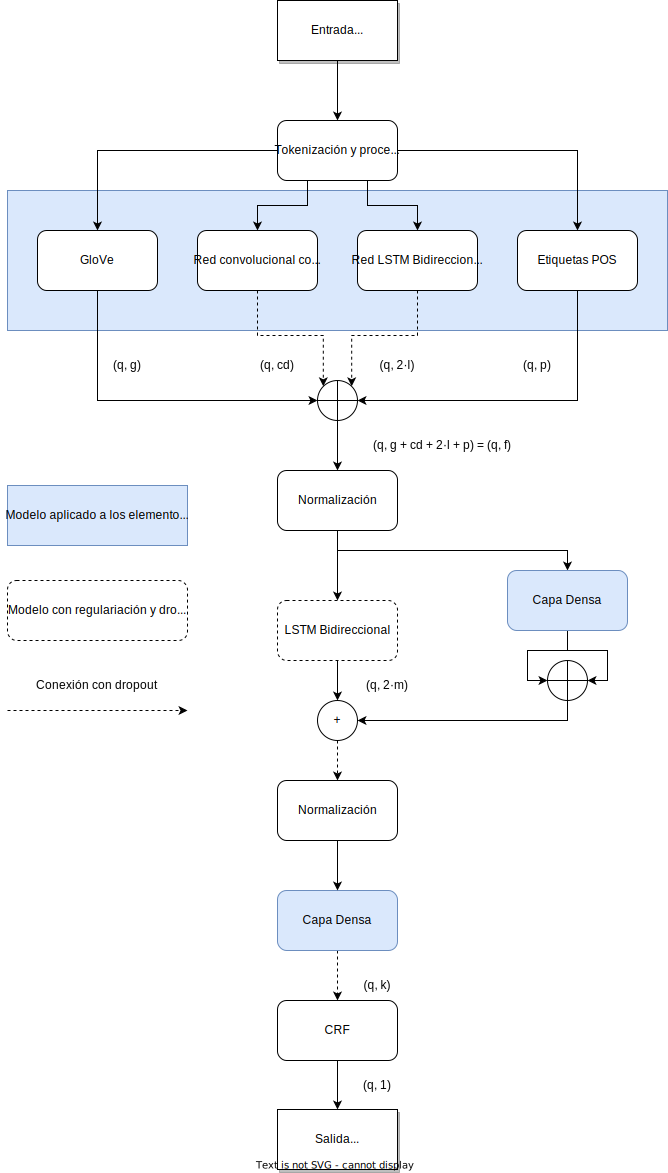
\includegraphics[scale=.3]{Graphics/Modelo_Segmenter_UDA.png}
            % \includesvg[options]{Graphics/Modelo Segmenter UDA.svg}
        \end{center}
	    \caption{Segmentador UDAs}\label{fig:seg_uda}
	\end{center}
\end{figure}

\subsection{Posporcesamiento}

La salida del modelo constituye una secuencia de etiquetas en formato BIOES. La secuencia devuelta puede que contenga
errores en la estructura BIOES, por ejemplo, secuencias no terminando en E, segmentos continuos con más de una meta-etiqueta.
Para la corrección de la estructura se propone el siguiente algoritmo, el cual se divide en dos partes. La primera
parte consiste en arreglar la estructura BIOES, para esto se mantiene una ventana de tamaño
3 sobre la secuencia y asume que la parte anterior a la posición de la ventana no presenta errores, al encontrar una
ventana inválida se necesita observar la siguiente ventana para poder decidir cómo se arregla el error ya que se
podría dar el caso de OOI OIO, en donde solamente viendo la primera ventana no se podría saber si el cambio 
correcto corresponde a sustituir I por B o por S. Una vez observado las dos ventanas se procede a realizar el 
arreglo correspondiente. En casos donde sea ambigua la manera de arreglar la ventana, IIO (La I o la O pueden ser 
sustituidas por una E) por ejemplo se utiliza una función que recibe un segmento y devuelve la gravedad del error,
el error con mayor gravedad será arreglado, en caso de ser iguales se arreglará la etiqueta más a la izquierda.
Este procedimiento devuelve una secuencia BIOES correctamente anotada, debido a que a partir de una secuencia sin 
errores en cada paso se va arreglando la ventana y una vez esta llega al final arregló todos los elementos de la secuencia.
Una vez se tiene la secuencia tiene la estructura BIOES correctamente anotada el problema
consiste en arreglar las meta-etiquetas, ya que una misma secuencia BIOES pudo haber sido anotada con diferentes
tipos, en este caso se toma la etiqueta más representativa de la secuencia.

\section{Predicción de enlaces}

Este modelo consiste en dados dos pares de UDA previamente extraídas, 
extraer y clasificar la relación entre ellas, como tarea auxiliar se realiza además la clasificación 
de las UDAs. Su salida consiste en una tupla conteniendo las clases de relación, tipo de UDA fuente y 
tipo de UDA objetivo respectivamente $(r \in R, s \in U, t \in U)$ donde $R$ y $U$ son los conjuntos de 
posibles tipos de relaciones más una clasificación que representa que no están relacionadas y los tipos de UDAs 
del corpus con que se entrena.

\subsection{Modelo}

Sea dos UDAs, $S$ y $T$, una representa la fuente de la relación, mientras que la otra representa
el objetivo. Estas secuencias son tokenizadas y se les asigna la representación \textbf{GloVe} de cada palabra, obteniendo
dos vectores de dimensión $u \times g$, donde $u$ es el tamaño máximo de UDAs en el conjunto de entrenamiento.
Estos vectores son modificados por una red densa compuesta por $ca$ capas con activación \textbf{relu}. 
Al finalizar este procesamiento se añade una conexión residual
a la salida. El próximo paso consiste en aplicar una capa densa de dimensión $di$ y luego un \emph{average pooling}
de tamaño $dp$, obteniendo vectores de dimensión $\frac{q}{di} \times dq$. 
Estos vectores son modificados por un \textbf{LSTM} bidireccional con $lm$ unidades. Un módulo de atención es aplicado 
sobre los vectores fuentes, 
en este actúan como consultas el promedio de los vectores objetivo y como llaves y valores los vectores fuentes,
el procedimiento simétrico es realizado para los vectores objetivos.
La salida de los procesamientos son concatenados con la distancia argumentativa obteniendo una representación 
conjunta de la relación a analizar. Esta representación conjunta es modificada por una red residual obteniendo
una representación final de dimensión $ff$ y luego sometida a los clasificadores de relación y de tipos de UDAs.

\begin{figure}[h!]
	\begin{center}
		\begin{center}
			\includegraphics[scale=.3]{Graphics/Modelo_Link_Prediction.png}
            % \includesvg[options]{Graphics/Modelo Link Prediction.svg}
        \end{center}
	    \caption{Predictor de enlaces}\label{fig:link_predictor}
	\end{center}
\end{figure}

Para prevenir el sobre ajuste se agregaron capas de normalización y de \emph{dropout} entre cada proceso y se usaron regularizaciones
L2 y \emph{dropout} en las capas densas y \textbf{LSTM}. Para prevenir el sobre entrenamiento se aplicó una 
terminación temprana de este cuando no se enontraba una mejora de la función de pérdida en el conjunto de validación.
Como optimizador se utilizó Adam con descenso exponencial.
